In this chapter we introduce the project by providing a broad overview of the reason why this topic has been chosen, consideration of various state-of-the-art technologies available for executing the research and the definition what result we expect to get from this report.

\section{Motivation}

The field of 3D computer graphics has always been a fascinating subject to me. Creating virtual worlds and being able to inspect those from every possible viewpoint is a great way to present almost any object one can think of to a wider audience. I finished my apprenticeship as a A/V media designer, so computer graphics are a helpful tool to e.g. previsualize camera work. The best fact about 3D is that it has so many versatile applications in many fields. 3D information can be retrieved from 2D images, taken with a real photo camera, via photogrammetry and can, in turn, be rendered onto a flat computer screen by rendering a three-dimensional scene with a virtual camera. At the point a object is available as a 3D model, it can be postprocessed in various ways. It can be animated, physically simulated and eventually rendered as a video. With modern display technologies the movie can be played out as a stereoscopic one and viewed with anaglyph (red, cyan), polarized, shutter or even without glasses by using e.g. a parallax barrier display (Wikipedia, \parencite{wiki:ParallaxBarrier}). Furthermore objects can become tangible via 3D printing or can be inspected interactively in games with the help of virtual reality glasses like the Oculus Rift (Oculus VR, \parencite{OculusVR}). It is amazing that anyone can create and enjoy those virtual worlds today.

Additionally, I am highly interested in historical topics. As an active member of a local citizens association and representative of a settlement, where I am always available for any citizenship matters that people might have, I get to know many interesting people and the projects they are working on. Thus I am learning a lot about interesting historical facts and development of culture. Of course, not only about positive history. Especially the history of the place where I live, Langwasser, district of Nuremberg, Germany, is very terrifying and shocking. The district has been formerly used for tent cities and the Märzfeld ("March Field", a representation and parade ground) during the Reich Party Congress in Nuremburg, Germany, between 1933 and 1938 (Wikipedia, \parencite{wiki:NaziPartyRallyGround}). The construction of a railway station, called Bahnhof Märzfeld which is located right in the center of Langwasser, was partly finished in 1938. That station has been used initially to transport the members of the Reich Party Congress to the event. During World War II it was used for the deportation of about 940 people to concentration camps, where only 17 of them survived (Stadtteilforum Langwasser, \parencite{StadtteilforumTafel6}). This railway station is in a ruinous condition at the moment. People go by without noticing that this is real history that passes them by. This was a big concern for me, so I started to search for ways to present history in a modern way, making it educational on the one hand and enjoyable on the other hand.

Consequently, there was the day I talked to my professor, Mr. Dr. Stefan Röttger, about my wish to use laser scanning for historic 3D reconstruction. Suprisingly my professor told me, that we have a laser scanning device at university which could be used for a thesis. The moment he told me that, was the moment I made my decision to center my thesis around laser scanning.

Lastly, a strong motivational force was discovered after researching how the laser scanner point cloud can be used to create the historic building model based off of a recent laser scan. 3D software enables a user to tweak automatically generated meshes or even to add new geometry. Due to my personal experience with the open source 3D graphics suite Blender and the decreasing interest in other software like Autodesk 3ds Max or Maya in favor of Blender (Google Trends, \parencite{Interest3DSoftware}) I decided to use Blender for the 3D modeling and animation part of this research. According to the trend it is a better option since it is being used by a greater number of artists and therefore future work will be of help to a lot of people. In addition, the source code of Blender is open. Any research based on it might benefit other researchers. Thus, it was necessary to be able to work with laser scanner output, namely point clouds, in Blender. Unfortunately Blender is not designed to work with point clouds at the time of this writing. This research should adress this issue by providing a way to complete the laser scanning production pipeline for artists who want to use Blender.

As will be described in greater detail hereafter, the aforementioned facts lead to an initial project specification. 

\section{Initial project specification}

The idea for this research started with the personal concern of reconstructing a historical site like the old railway station in Langwasser in its historic state. Due to the fact that this railway station has never been fully finished and therefore poor historical documentation, a 3D reconstruction wouldn't be complete. Luckily the famous Pellerhaus was the perfect candidate for this research\footnote{Amount of historical photos: Bahnhof Märzfeld: 9; Pellerhaus Nürnberg: 190}. After its destruction during World War II, it was rebuilt quite differently to the original state. While the inner courtyard is almost finished with reconstruction at the time of this writing, the facade is still looking modern. At that point, it was clear that the main research topic is going to examine ways to reconstruct the Pellerhaus facade in its historic state.
A more concrete specification was defined by considering how this is going to be done. The current state of the building has to be captured with laser scanning technology to get the correct measurements from the real world reference. We use a FARO Laser Scanner Focus\textsuperscript{3D} X Series device for this project.
This point cloud data needs to be processed then. To do so, a custom software is required to be written, which can read a file format exported from the proprietary FARO SCENE application, create a panoramic image representation of the data, use it to generate a 3D mesh surface and export this mesh to a widely supported file format. This research will mostly rely on the open source software Blender to model and animate the historic state of the Pellerhaus, thus it is crucial to provide a compatible output to be used as a basis for the design process. By creating a textured surface from the point samples, this research will provide a way for the artist to overcome a bad design decision in Blender, which is making it not capable of displaying or rendering colored point clouds at all (see thread by author on BlenderArtists \parencite{webBlenderArtistsPointCloudSupport} ). The goal of this research is to get a 3D model of the Pellerhaus in its historic state from 1605 by utilizing point clouds generated via laser scanning as described before.

\section{Project schedule}

This project is divided into two main phases. The first phase is developing the software for converting laser scanner point clouds as 3D panorama meshes. The second one is designing the historic 3D model from this initial mesh.\\

This is visualized in the following GANTT chart:\\

\definecolor{RoyalBlue}{RGB}{92,102,149}
\definecolor{OliveGreen}{RGB}{51,151,102}
\definecolor{Maroon}{RGB}{180,20,53}
\begin{ganttchart}[
	x unit=1.3cm,
	y unit title=0.7cm,
	y unit chart=0.8cm,
	vgrid, hgrid,
	time slot format=isodate-yearmonth,
	compress calendar,
	title/.append style={draw=none, fill=RoyalBlue!50!black},
	title label font=\sffamily\bfseries\color{white},
	title label node/.append style={below=-1.6ex},
	title left shift=.05,
	title right shift=-.05,
	title height=1,
	bar/.append style={draw=none, fill=OliveGreen!75},
	bar height=.6,
	bar label font=\normalsize\color{black!50},
	group right shift=0,
	group top shift=.6,
	group height=.3,
	group peaks height=.2,
	bar incomplete/.append style={fill=Maroon}
	]{2015-01}{2015-07}
	\gantttitlecalendar{year, month=shortname} \\
	
	\ganttset{progress label text={}, link/.style={black, -to}}
	\ganttbar[progress=100, name=pp]{Laser Scanning}{2015-01-15}{2015-01-25} \\
	
	\ganttgroup{Software development}{2015-02-15}{2015-06-10} \\
	\ganttbar[progress=100, name=T1A]{Import}{2015-02-15}{2015-02-18} \\
	\ganttbar[progress=100]{Processing}{2015-02-19}{2015-03-25} \\
	\ganttbar[progress=100, name=T1C]{Export}{2015-03-24}{2015-04-01} \\
	\ganttbar[progress=100]{Testing / Bugfixing}{2015-02-26}{2015-06-10} \\
	
	\ganttgroup{Video production}{2015-06-08}{2015-07-10} \\
	\ganttbar[progress=100, name=T2A]{Modeling}{2015-06-08}{2015-06-10} \\
	\ganttbar[progress=100]{Animation}{2015-06-10}{2015-07-02} \\
	\ganttbar[progress=100]{Rendering}{2015-06-12}{2015-07-10} \\
	
	\ganttset{link/.style={OliveGreen}}
	\ganttlink[link mid=.4]{pp}{T1A}
	\ganttlink[link mid=.159]{T1C}{T2A}
	\label{tab:project_schedule}
\end{ganttchart}\\


\section{State-of-the-art methods for 3D reconstruction}

There are several methods that allow for the generation of 3D meshes from various data. One can either use several still images or videos, sample the real world with modern sensor technology or use open data for generating geometry of varying complexity. This is described as follows:

\subsection{Light Detection And Ranging (LiDAR)}

The term Light Detection And Ranging (in short LiDAR) is commonly used with high precision applications, such as scanning and mapping of indoor and outdoor environments. It uses a laser beam emitter and receiver. By using the Distance-Speed-Time formula it is very easy to compute how far away an object is:\\

$$  speed = \dfrac{distance}{time} \Longleftrightarrow distance = time * speed $$\\
The time between sending a signal and receiving it is measured and multiplied by the speed of light ($c = 299,792,458 \medspace \frac{m}{s}$, Wikipedia \parencite{wiki:SpeedOfLight}). This returns the meters the light traveled from the emitter to the obstacle and back. Dividing this distance by two yields the range to the obstacle in meters (Schroeder \parencite[see][p8-9]{dp_lidar}).

As this gives the meters to only one specific point, it is necessary to keep measuring from different view orientations. This can be done by rotating the scanning device horizontally and vertically simultaneously. To avoid mechanical imprecision or cables from winding up most devices usually use one motor for the horizontal and another motor to control a flat mirror on an elliptical mount for the vertical rotation. That way it is possible to sample a lot of points around the device position quickly and effectively.

\begin{figure}[h]
	\centering
	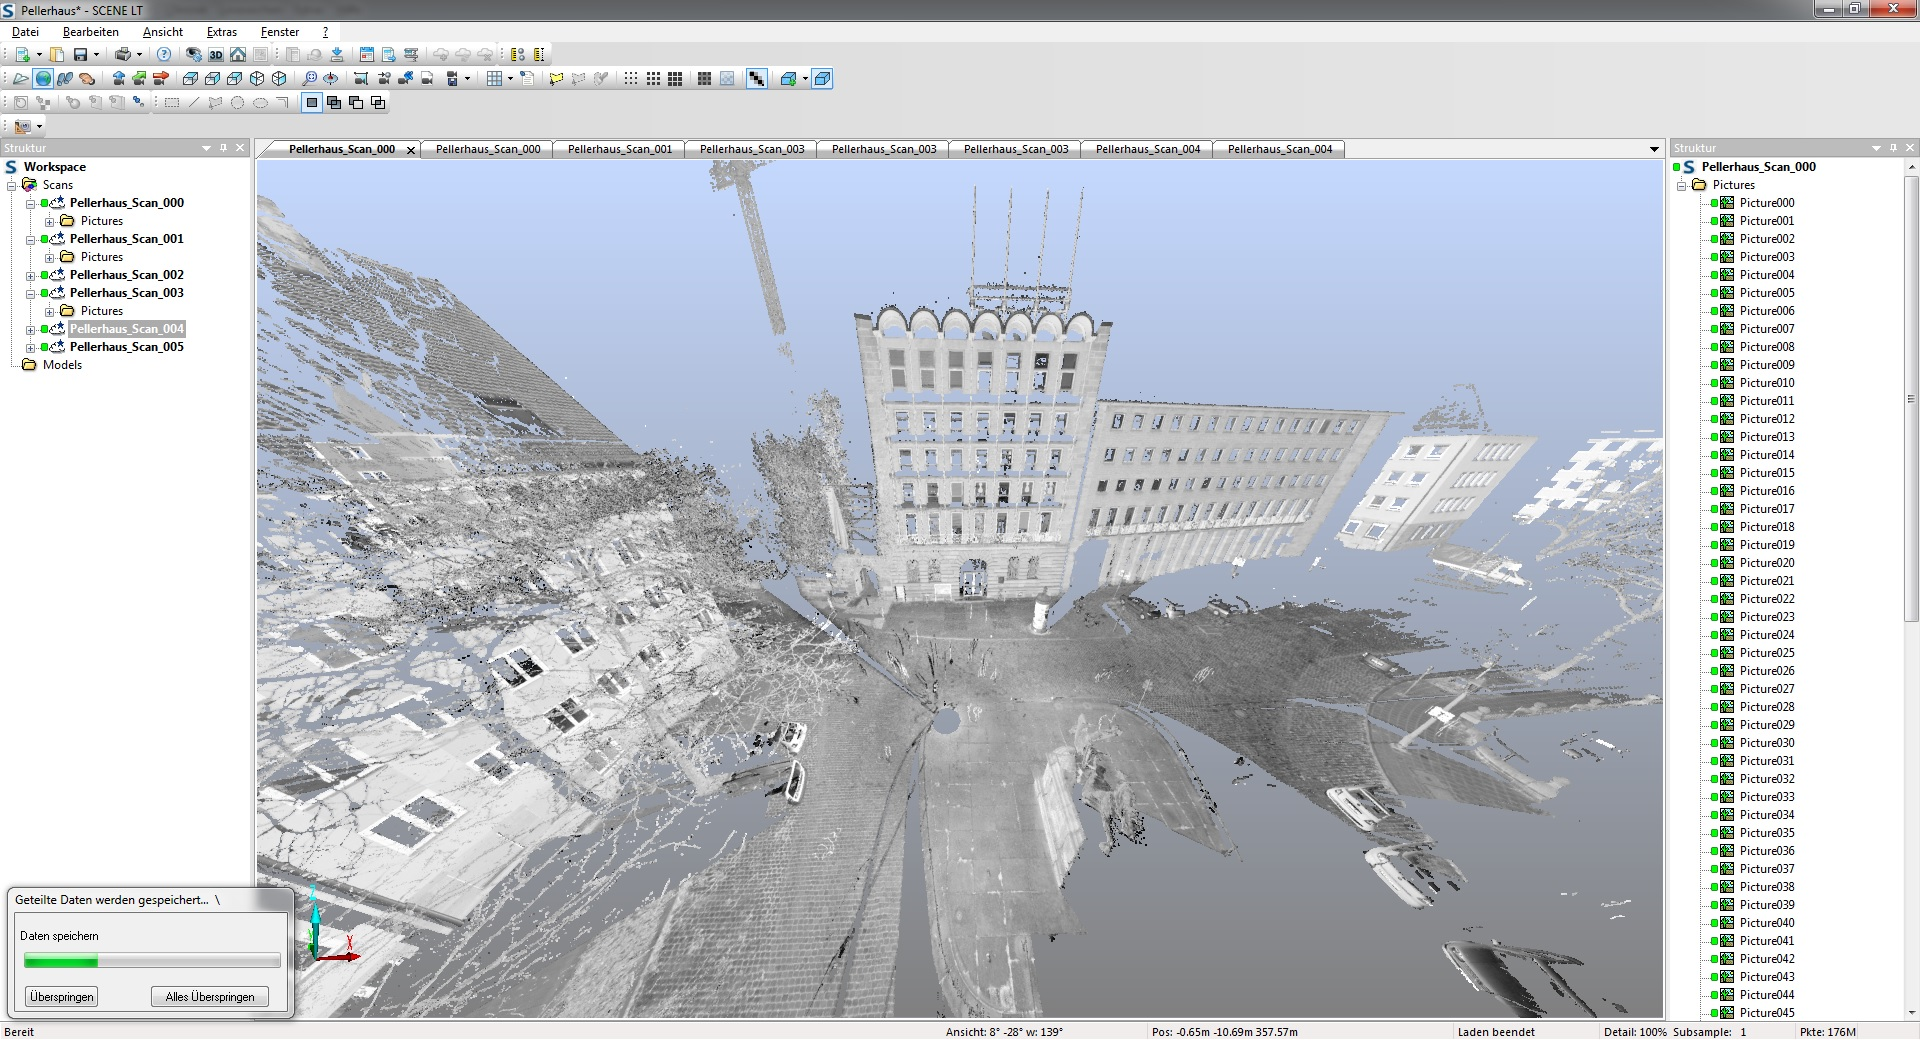
\includegraphics[scale=0.25]{Pellerhaus_FirstGlance.jpg}
	\caption{LiDAR Scanner Point Cloud of the Pellerhaus}
	\label{fig:LiDAR_PointCloud}
\end{figure}

In this work the LiDAR scanner FARO Focus\textsuperscript{3D} is being used. It is capable of capturing 976,000 points per second with a vertical and horizontal field of view of 305 and 360 degrees, respectively (Techsheet FARO Focus\textsuperscript{3D}, \parencite{faro_techsheet}). For allowing a better registration additional sensors can be used such as GPS for localization and a barometer for height measurement. The measured points can be colored using an automatic color overlay from a built-in camera at a 70 megapixel resolution. The price for the Focus\textsuperscript{3D} totals at 61,404.37 Euro (Opti-cal Survey Equipment Ltd. \parencite{survey_equipment}).

Besides using a stationary device, portable devices are also available. Recently a new technology has been revealed by Csiro and is called \textit{Zebedee}. This handheld laser scanner can be used in challenging environments where a stationary device would require several scans to cover the whole area (e.g. caves, staircases) while the operator is walking. It samples over 40,000 range measurements every second and consists of a 2D laser scanner mounted on a spring system (Mail Online, \parencite{zebedee_info}). Especially the visual effects field has a great use for this device, since the environments can vary a lot during video shootings and a 3D mesh representation is ubiquitous today. The price for the ZEB1 handheld laser scanner is 17,000 Euro\footnote{Source: Personal contact to sales team}.

Although measuring with laser technology can be found in household devices as an alternative for tape measuring, it is still quite complicated to reverse engineer such devices to get the raw distance reading. Fortunately a group of engineers tried to bridge the gap by starting a crowd funding campaign for a low-cost laser range finder, called the LiDAR-Lite (PulsedLight \parencite{pulsedlight}). It has a total range of 40 meters with a resolution of 1 cm. During this research this sensor is being used with a custom arduino build to examine how it can be used as a cheap alternative to the examples mentioned in the beginning. The price for one module is at 82 Euro.

\subsection{Ultrasonic}

In contrast to LiDAR, most ultrasonic sensors are cheap, but generally are not used for higher distances at several tens of meters (though, there are products for a range higher than 100 meters, compare VEGAPULS 69 \parencite{vegapuls}). The reason for this is that sound is usually affected stronger by environmental properties than light (compare Sensors Magazine \parencite{sensorsmag}). Due to this they are often used for shorter distances e.g. for near field obstacle recognition in robotics or in small desktop laser scanners (compare Dinh \parencite{yt_smalldesktoplaser}). Typical ultrasonic sensor modules with a maximum range of around 5 m can be purchased for 5 Euro already.



\subsection{Photogrammetry}

Photogrammetry (also referred to as multi-view reconstruction) is a technique from the Computer Vision field and presents a cost-effective alternative to laser scanning. A real 3D object can be reconstructed as a virtual 3D model by using photographs of the scene and feeding them into such software. This works by detecting image features (for example by using Harris Corner Detector or SIFT algorithms), matching those between image pairs, computing the respective camera positions and re-projecting the reconstructed 3D points to get a point cloud representation of the real photograph (compare Solem \parencite[][p29]{bookProgrammingComputerVisionwithPython}).
The Computer Vision algorithms get better each day and there is plenty of software using them. Basically we can distinguish between open source, free or commercial software for this task. Usually open source software can be free to use, too. Though, it might have some limitations defined by its license, e.g. only granting non-commercial use. On the contrary, some licenses even allow users to sell the software under a different brand name as is the case with e.g. Blender. In this example the GNU GPL Version 3 license allows a company to sell Blender with prices starting at 47 Dollar. As this is only a side note, more information on that topic can be found in \parencite{blender_rebranding}.
To compare the results of open source and commercial photogrammetry software we processed 356 photos of the Pellerhaus with two applications. On the one hand VisualSFM for generating a sparse point cloud in conjunction with CMP-MVS for the dense point cloud generation via open source tools have been used. On the other hand the commercial software Agisoft Photoscan Professional was used which costs 3,499 Dollars but can be tested with a fully functional 30 day trial, like in this research.

\begin{figure}[h]
	\centering
	\begin{subfigure}[b]{1.0\textwidth}
		\centering
		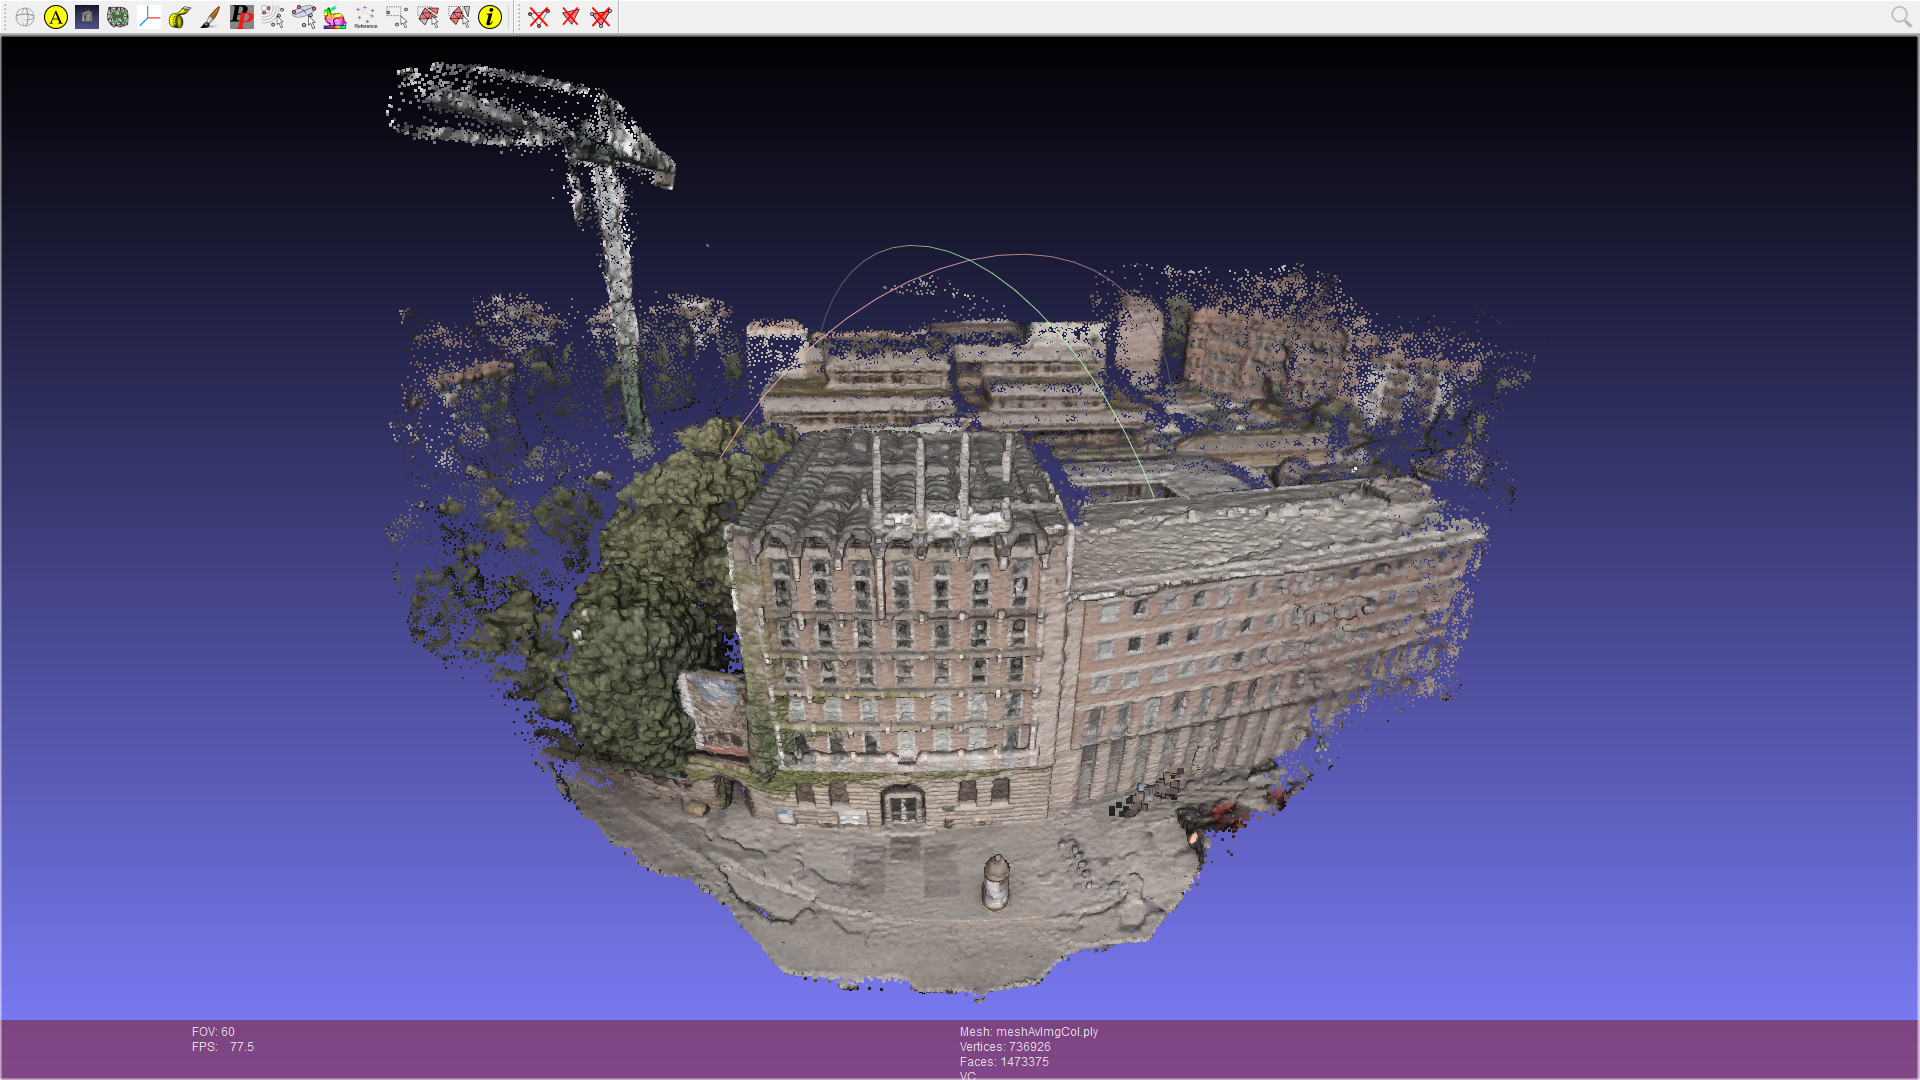
\includegraphics[width=\textwidth]{Photogrammetry_VisualSFM.jpg}
		\caption{Open Source: Visual SFM + CMP-MVS (736,926 points)}
		\label{fig:visualsfm}
	\end{subfigure}
	\hfill
	\begin{subfigure}[b]{1.0\textwidth}
		\centering
		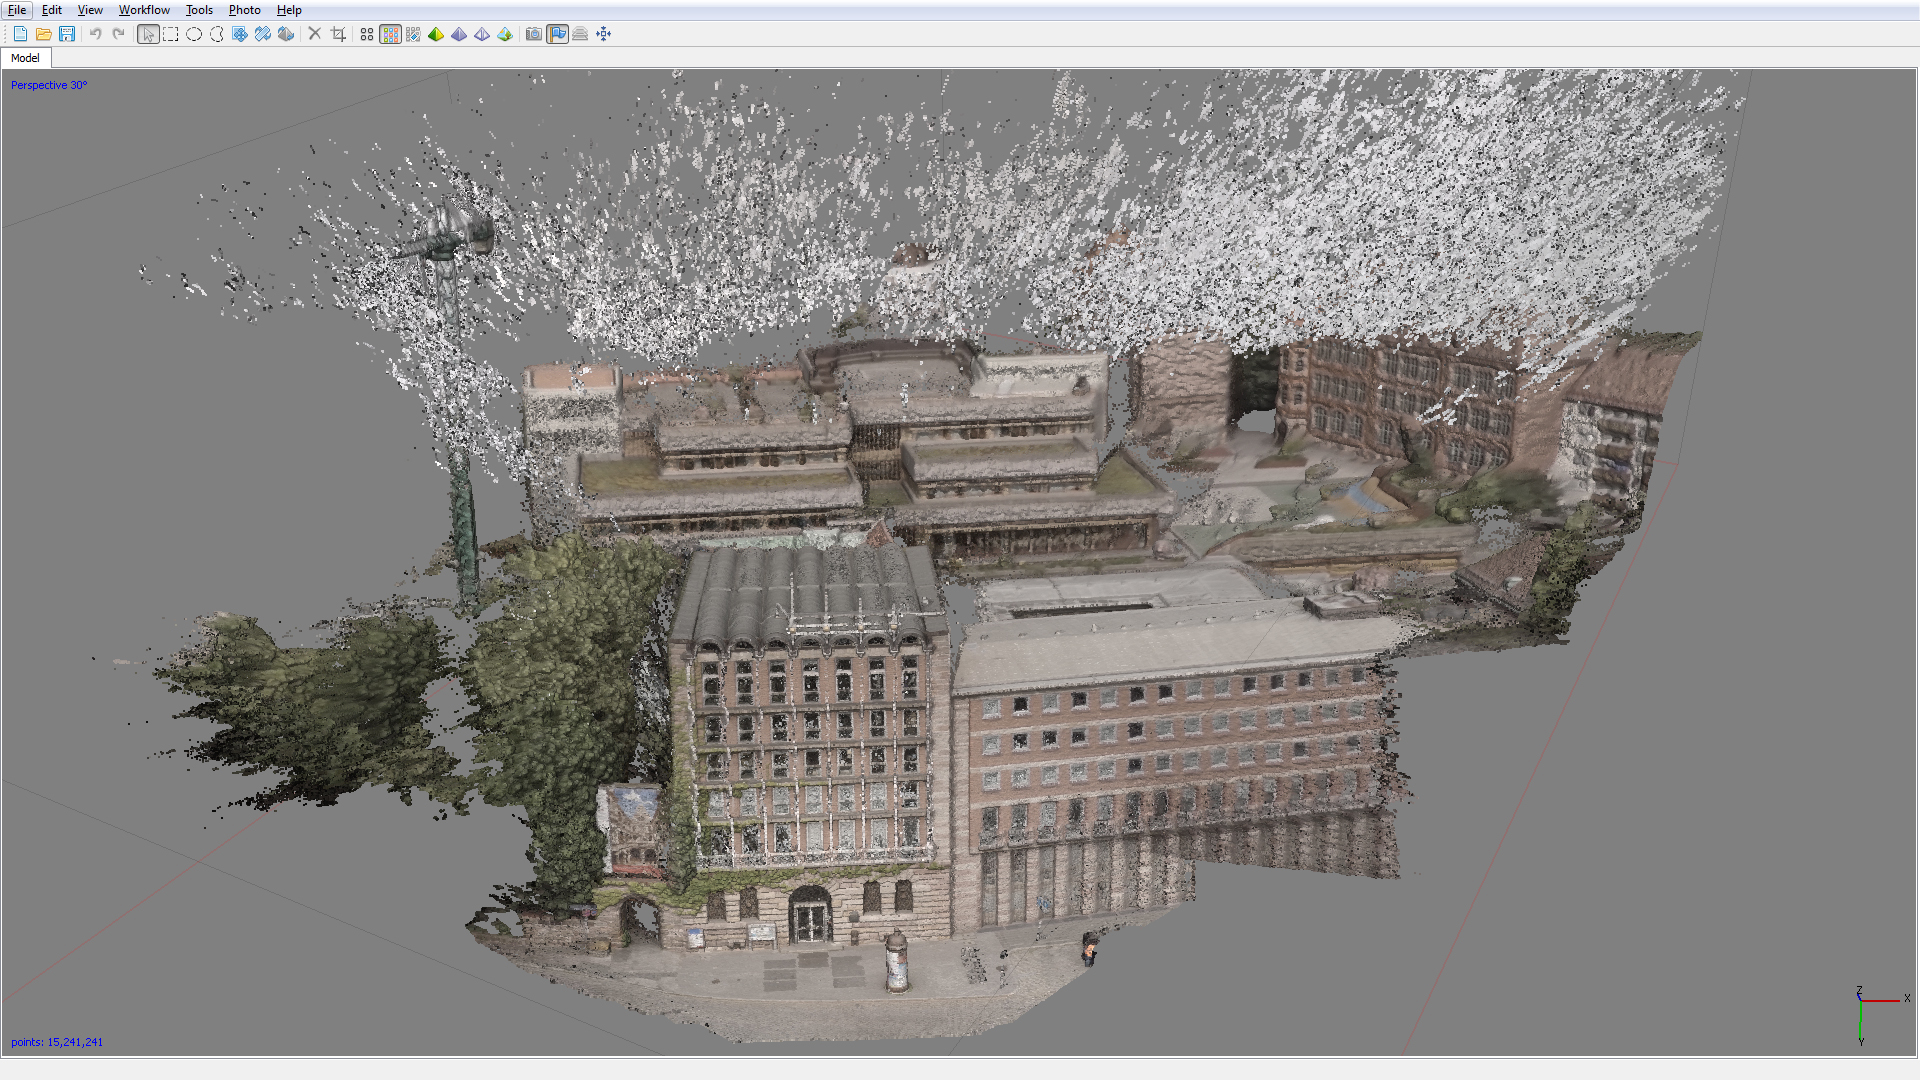
\includegraphics[width=\textwidth]{Photogrammetry_Agisoft.jpg}
		\caption{Commercial: Agisoft Photoscan (15,241,241 points)}
		\label{fig:photoscan}
	\end{subfigure}
	\caption{Multi-view reconstruction point clouds generated from 356 photos}
	\label{fig:multiview reconstruction pellerhaus}
\end{figure}

Comparing the results, the point cloud output from Agisoft Photoscan is much more detailed, approximately by a factor of 20. Furthermore VisualSFM created a bent facade, whereas Photoscan preserved all important straight lines. All in all it can be observed that the algorithms of Photoscan are more sophisticated and suited better for images taken with a great amount of lens distortion, though this is something that should be avoided when considering using the footage for multi-view reconstruction (see Balletti et al. \parencite{calibration_of_action_cameras}). Both applications generate a model that can provide a good initial mesh of a scene, but the computation takes very long. Photoscan was using all ressources of an eight core Intel i7 workstation with 16 of RAM running for about 4 days.

Photogrammetry will be used in this project to try reconstructing surfaces from historical images. Fortunately historical stereographic image pairs are provided through the Altstadtfreunde Nürnberg e.V. By matching the laser scanner data with the Photogrammetry output a good groundwork is expected to be done for the final surface reconstruction.

\subsection{Depth Cameras}

Instead of using photogrammetry software to retrieve 3D information from images, Depth Cameras can be used which encompass the same functionality in hardware. Popular devices are e.g. the Microsoft Kinect v1 and v2 or the Asus Xtion Pro Live, typically ranging between 100 and 200 Euro. Using stereo matching algorithms those devices can determine the distance, or depth, of a certain point. First, an infrared projector emits a speckle pattern which an infrared camera analyzes to match points between the emitter and projector. By using a mathematical process based on trigonometry called Triangulation (compare Wikipedia \parencite{wiki:Triangulation}) it is possible to calculate the distance to a point if certrain properties are known, such as the distance of a fixed baseline between two observing points and the angle from the baseline to the observed point. There are some problems known with those sensors which limit their use mostly to indoor applications. Direct sunlight can wash out the speckle pattern or multiple sensors can confuse each other. Despite those issues Depth Cameras provide a simple and fast way to get 3D point clouds of real objects. Custom software can be written and access this data directly from the depth sensor. The Microsoft Kinect SDK provides some examples how this can be accomplished and the Kinect Fusion project presents a complete solution for creating 3D surfaces of high resolution in real-time (see Newcombe et al. \parencite{kinectfusion}).

\subsection{Google Maps \textsuperscript{\textregistered} }

The commercial application allows viewing cities from the sky with a rough representation of 3D building shapes (compare Zamora \parencite{google_maps}). While this service had gray boxes some years ago, today the visualization is getting more accurate. Nowadays it is possible to see small details with better modeled and textured buildings.

\subsection{Open Street Map \textsuperscript{\textregistered} }

The open source alternative to the commercial service above offers the basic functions for map viewing and navigation. OpenStreetMap (OSM) offers very detailed access to its data, like boundaries, streets and building footprints. That way it is possible to extract simple building shapes (compare F4 \parencite{f4map}) that can be used in custom software free of charge.

To allow for a better mapping of buildings there are also proposals on an indoor version of OSM (compare OpenStreetMap Wiki \parencite{openstreetmap_wiki}). Having this data available is a helpful asset for various applications such as indoor navigation at railway and subway stations, mobile emergency exit information and robotics.

\subsection{Bavarian State Office for Survey and Geoinformation}

Geodata and city plans are usually provided officially through governmental institutions. They provide various types of data, among others historical aerial photographs, digital elevation models (DEM) and also 3D building shapes. For educational purposes (like i.e. this research) they offer a university discount for the data of 25 percent. A usual dataset without any discounts containing 7580 buildings of Langwasser, district of Nuremberg in Germany, costs 1,158 Euro\footnote{Personal research and contact}.

\subsection{Autonomous mapping with UAV's and SLAM}

Drones, or unmanned aerial vehicles (UAV's), are getting more popular each day. Most of them are also equipped with a camera which allows for taking pictures or videos from viewpoints a human cannot reach easily. More expensive drones have LiDAR systems attached (Shen et. al. \parencite{drones_lidar}) which allow - together with the IMU (Inertial Measuring Unit) and GPS (Global Positioning System) to localize it and map its environment. A popular term for retrieving the current position based on various sensor data while creating a virtual representation of the environment at the same time is Simultaneous Localization And Mapping (SLAM).

\subsection{Manual methods}

If all other methods fail, there is still the chance to get a reconstruction done roughly by taking measurements of real objects with measuring tapes or eyeballing. Loading reference pictures from the front, side and top view into a 3D software can already yield decent results. Furthermore this is the standard way a 3D artist would begin to model a digital human or character that a concept artist provided by sketching those three main views of it. Concept art that is accurate and matches every other view can help a 3D artist to block out the shapes very fast. In certain circumstances it can even be faster than setting up a scanning environment or generate a mesh via photogrammetry, because the generated meshes need to retopolgized (that is, re-modelled with a strong focus on the clean layout of the mesh grid) anyway as soon as they are considered to be e.g. used in animation.

\section{Defining the scope of this research}

Although this work uses a combination of several techniques (briefly presented above), the main focus is put on examination if panoramic projection and meshing of laser scanner point clouds will be an aid for 3D reconstruction or not. This will be evaluated by using the result from the custom converter software in a real world use case of using the generated mesh in the design process.